\documentclass[letterpaper, 10pt]{article}
% \usepackage{minipage}
\usepackage{graphicx}
\usepackage{graphics}
\usepackage{hhline}

\usepackage{geometry}
\geometry{letterpaper, margin=0.75in}
\usepackage{array}

\usepackage{amsmath,amsfonts}
\usepackage{amssymb, amsthm}
\usepackage{mathtools}
\usepackage{dblfloatfix}
\usepackage{float,color,graphicx}
\usepackage{tikz}
\usepackage{verbatim}
\usetikzlibrary{calc}
\usetikzlibrary{patterns}
\usepackage{pgfplots}
\usepackage{enumitem}
\usepackage[font=footnotesize,skip=4pt]{caption}

\begin{document}

\newcommand{\pGap}{\em Potential Gap}
\newcommand{\saferGap}{\em Safer Gap}
\newcommand{\keyhole}{\em Keyhole ZBF}

\def\pgnt{PG$^-$}
\def\pg{PG}
\def\pgpo{PG+PO}
\def\pgp{PG+P}
\def\sgnt{SG$^-$}
\def\sg{SG}
\def\sgp{SG+P}
\def\pgm{PG+M}
\def\sgm{SG+M}
\def\sgmpo{SG+M+PO}

\title{Ablation Study Configurations and Results}
\maketitle

\section{Configurations}

Configurations of ablation study. {\pgp} and {\sgp} are not included in the manuscript since they only provide minor comparisons. A standard feedback and feedforward tracking controller is used to follow the time-varying trajectory. Let $g^W_R(t)$ be the current robot pose in the world frame and $g^{W,*}_R$ be the desired robot pose in the world frame. Define the pose error by
\begin{equation}
g_{\text{err}} = (g^W_R(t))^{-1}g^{W,*}_R
\end{equation}
Extract from $g_{\text{err}}$ the x-coordinate error $\Delta x$, y-coordinate error $\Delta y$, and the orientation error $\Delta \theta$. The commanded robot body velocity for nonholonomic robots is
\begin{equation}
\xi_{\text{com}} = 
\begin{bmatrix}
\nu \\
\omega
\end{bmatrix}
=
\begin{bmatrix}
k_{\text{drive,x}} & 0 & 0 \\
0 & k_{\text{drive,y}} & k_{\text{turn}}
\end{bmatrix}
\begin{bmatrix}
\Delta x \\
\Delta y \\
\Delta \theta
\end{bmatrix}
+
\begin{bmatrix}
\nu^*(t) \\
\omega^*(t)
\end{bmatrix}
\end{equation}
In the {\pgnt}, {\pg}, {\pgpo}, {\sgnt}, and {\sg}, there is no desired velocities $[\nu^*(t), \omega^*(t)]^T$ in the feedback controller.

\begin{figure}[h!]
\hspace{-0.8em}
\centering
\begin{minipage}{\columnwidth}
\small
\centering
\captionsetup{justification=centering}
\captionof{table}{Configurations of all planners in the ablation study\label{tab:ab}}
% \vspace{2in}
\begin{tikzpicture}[inner sep=0pt,outer sep=0pt,scale=1, every node/.style={scale=1}]
\def\labelp{P}
\def\labelb{B}
\def\labely{Y}
\def\labeln{N}
\def\labelpt{PT}
\def\labelmt{MT}
    \node[anchor=west] (sim_conf) at ($(0, 0pt)$)
    {
    \setlength{\tabcolsep}{2pt}
    \begin{tabular}{|c||c|c|c|c|c|}
    \hline 
    \textbf{Planners} & \begin{tabular}{@{}c@{}}Path \\ Planning \end{tabular}
    & \begin{tabular}{@{}c@{}}Feedback \\ Tuning \end{tabular}
    & \begin{tabular}{@{}c@{}}Projection \\ Operator$^*$ \end{tabular}
    & \begin{tabular}{@{}c@{}}Trajectory \\ Synthesis$^\dagger$ \end{tabular}
    & \begin{tabular}{@{}c@{}}Tracking \\ Method \end{tabular}
    \\ 
    \hline 
    \pgnt & \labelp & \labeln & \labeln & \labeln & \labelpt \\
    \pg & \labelp & \labely & \labeln & \labeln & \labelpt \\
    \pgpo & \labelp & \labely & \labely & \labeln & \labelpt \\ 
    \sgnt & \labelb & \labeln & \labeln & \labeln & \labelpt \\
    \sg & \labelb & \labely & \labeln & \labeln & \labelpt \\ 
    \pgp & \labelp & \labeln & \labeln & \labely & \labelpt \\
    \sgp & \labelb & \labeln & \labeln & \labely & \labelpt \\
    \pgm & \labelp & \labeln & \labeln & \labely & \labelmt \\ 
    \sgm & \labelb & \labeln & \labeln & \labely & \labelmt \\ 
    \sgmpo & \labelb & \labeln & \labely & \labely & \labelmt \\ 
    \hline 
    \end{tabular}
    };
    
    \node[anchor=north west] (t1) at ($(sim_conf.south west)+(1em, -0.5em)$) {\labelp: Potential Field};
    \node[anchor=west] (t2) at ($(t1.east)+(1em, 0em)$) {\labelb: Composite B\'{e}zier Path};
    \node[anchor=west] (t3) at ($(t2.east)+(1em, 0em)$) {\labely: Yes};
    \node[anchor=west] (t4) at ($(t3.east)+(1em, 0em)$) {\labeln: No};
    \node[anchor=north west] (t5) at ($(t1.south west)+(0em, -0.5em)$) {\labelpt: Pose-based Trajectory Tracking};
    \node[anchor=north west] (t6) at ($(t5.south west)+(0em, -0.5em)$) {\labelmt: NMPC Trajectory Tracking with {\keyhole}};

    \node[anchor=north west] (t7) at ($(t6.south west)+(0em, -0.5em)$) {$*$};
    \node[anchor=north west,text width=28em] (t8) at ($(t7.north east)+(0.3em, 0em)$) {{\pgpo} uses projection operator (PO) in every planning loop;};
    \node[anchor=north west,text width=25em] (t9) at ($(t8.south west)+(0em, -0.5em)$) {{\sgmpo} only needs PO if NMPC cannot converge within prescribed time.};
    
    % \node[anchor=north west] (t7) at ($(t6.south west)+(0em, -0.5em)$) {Trajectory Synthesis:};
    % \node[anchor=north west,text width=18em] (t8) at ($(t7.north east)+(0.4em, 0em)$) {generate time-varying trajectory with desired velocities.};
    \node[anchor=north west] (t10) at ($(t7.south west)+(0em, -3.3em)$) {$\dagger$ Generate time-varying trajectory with desired velocities.};

    \node[anchor=north west] (t11) at ($(t10.south west)+(0em, -0.5em)$) {$^-$ The feedback gains of path following are not tuned.};
    
\end{tikzpicture}
\end{minipage}
\vspace{-0.5em}
\end{figure}

\section{Benchmark Scenarios}

Four simulation scenarios shown in Fig.~\ref{fig:sim}. Start region/poses (red) and end region/poses (green) are labeled in sector and campus worlds. In the dense world, robots navigate from top to bottom. The start and goal poses are randomly chosen from the red points in the office world.

\begin{figure*}[htb]
 \vspace*{0.06in}
   \centering
   \begin{minipage}{0.22\textwidth}
   \centering
   \begin{tikzpicture}[inner sep=0pt,outer sep=0pt]
     \node[anchor=south west] (comp1) at ($(0, 0)$)
     	{{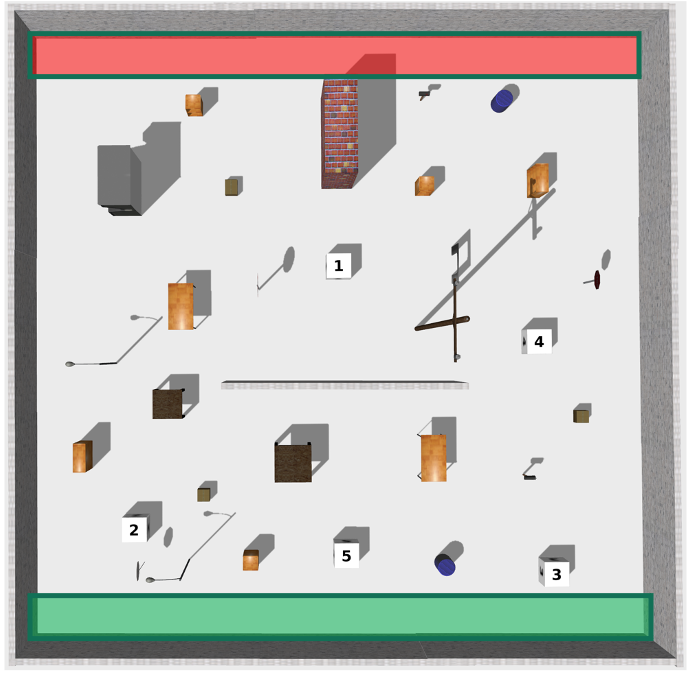
\includegraphics[height=1.4in]{figs/sce1.png}}};
     \node[anchor=north] at ($(comp1.south)+(0,-0.3)$) {\centering Sector};
   \end{tikzpicture}%
   \end{minipage}
   \hfill
   \begin{minipage}{0.22\textwidth}
   \centering
   \begin{tikzpicture}[inner sep=0pt,outer sep=0pt]
     \node[anchor=south west] (comp2) at ($(0, 0)$)
     	{{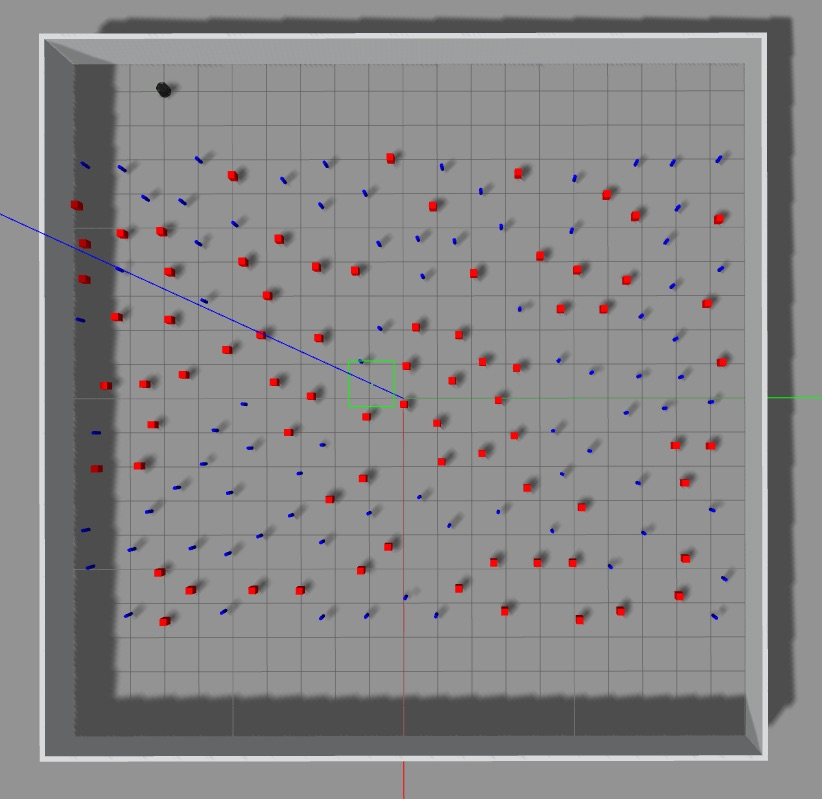
\includegraphics[height=1.4in]{figs/sce2.jpg}}};
     \node[anchor=north] at ($(comp2.south)+(0,-0.3)$) {\centering Dense};
   \end{tikzpicture}%
   \end{minipage}
   \hfill
   \begin{minipage}{0.22\textwidth}
   \centering
   \begin{tikzpicture}[inner sep=0pt,outer sep=0pt]
     \node[anchor=south west] (comp2) at ($(0, 0)$)
     	{{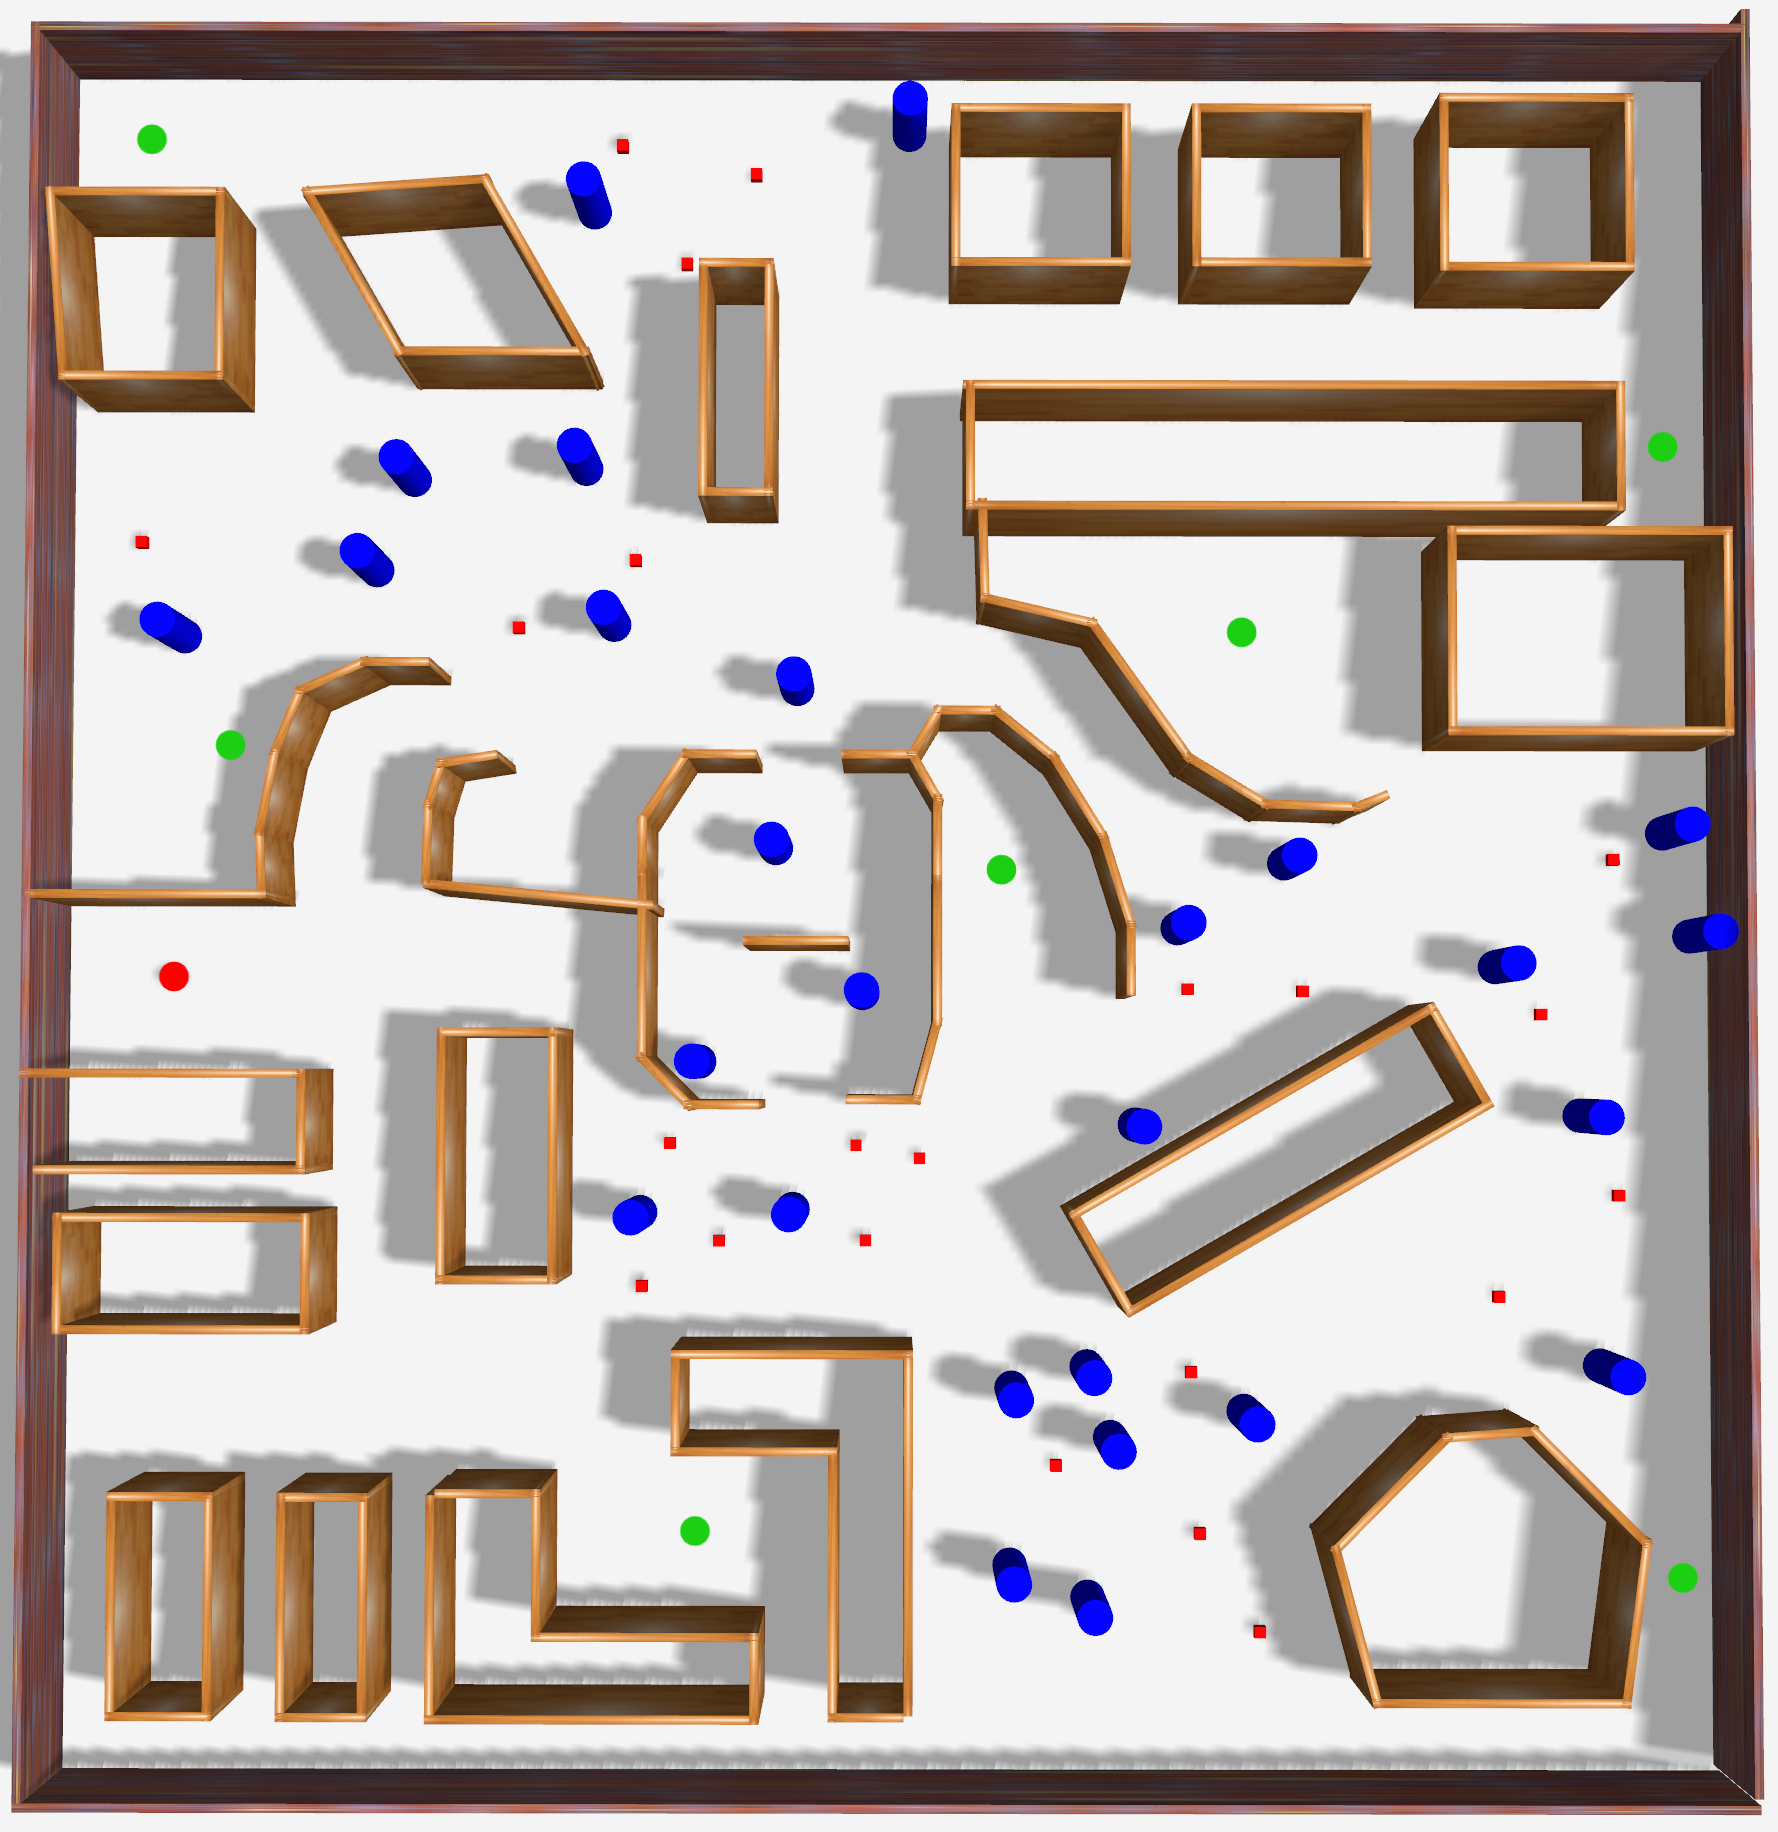
\includegraphics[height=1.4in]{figs/sce3.png}}};
     \node[anchor=north] at ($(comp2.south)+(0,-0.3)$) {\centering Campus};
   \end{tikzpicture}%
   \end{minipage}
   \hfill
   \begin{minipage}{0.3\textwidth}
   \centering
   \begin{tikzpicture}[inner sep=0pt,outer sep=0pt]
     \node[anchor=south west] (comp2) at ($(0, 0)$)
     	{{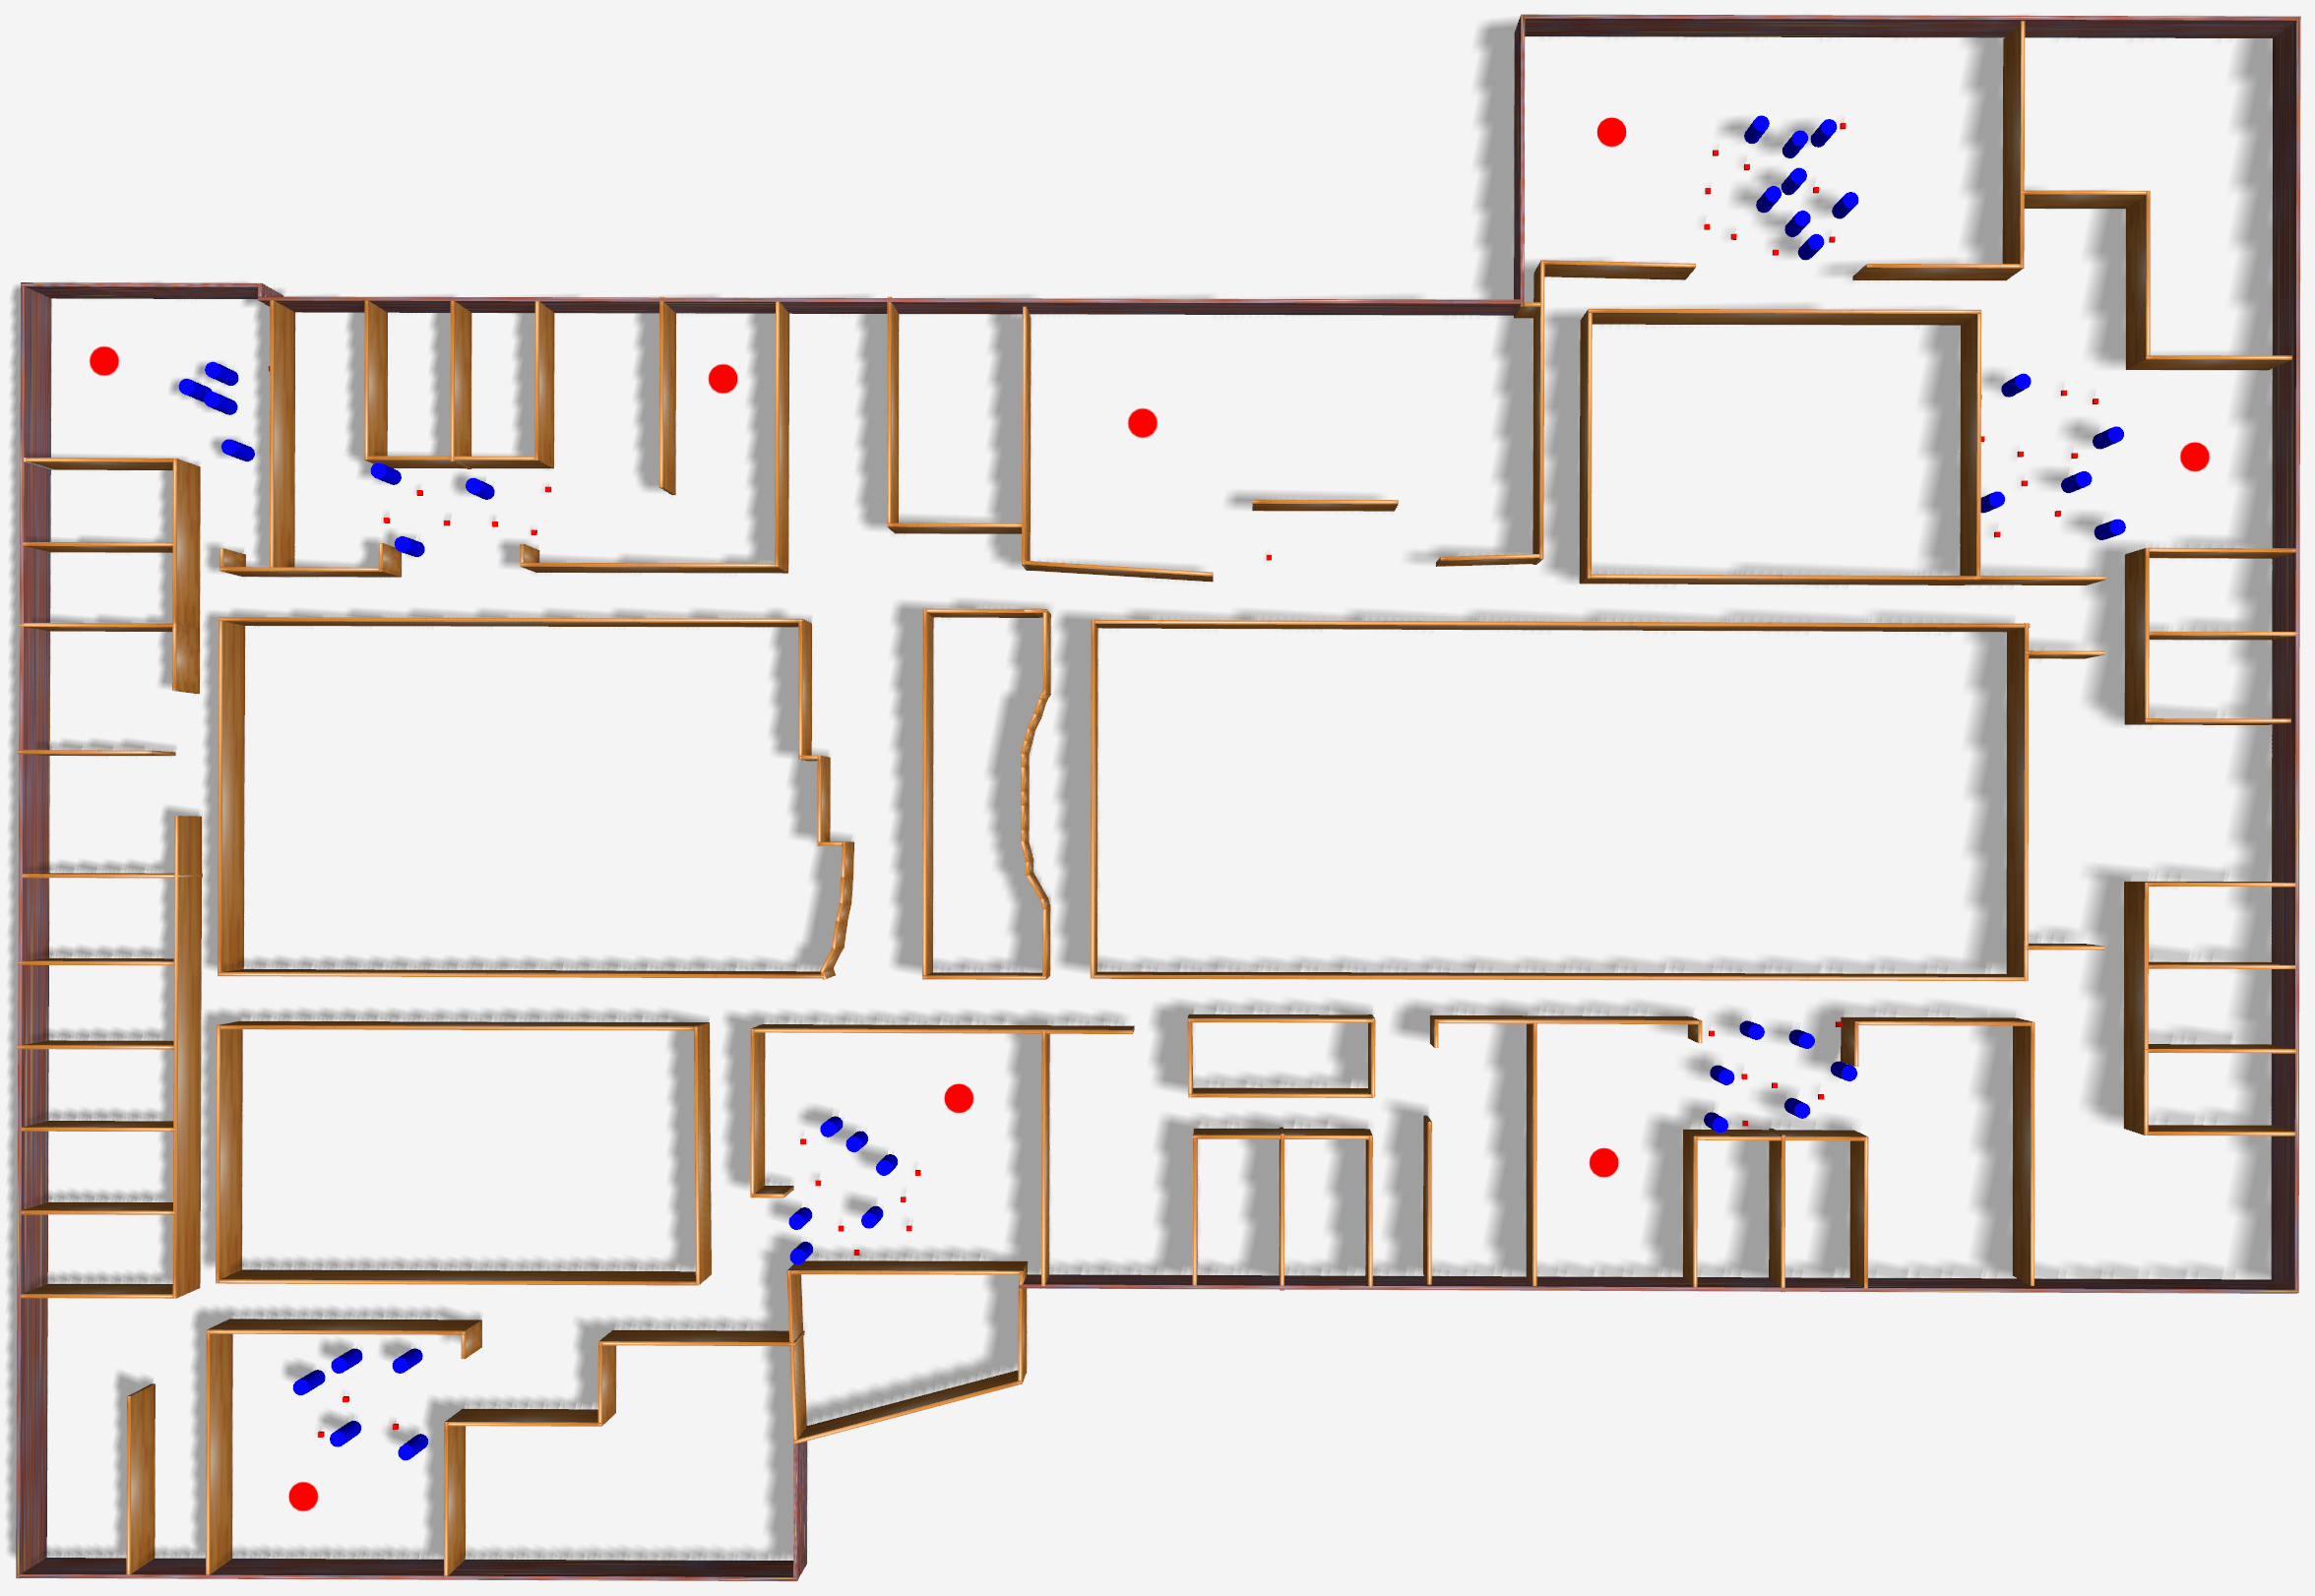
\includegraphics[height=1.4in]{figs/sce4.png}}};
     \node[anchor=north] at ($(comp2.south)+(0,-0.3)$) {\centering Office};
   \end{tikzpicture}%
   \end{minipage}
   \caption{Four simulation scenarios. Start region/poses (red) and end region/poses (green) are labeled in sector and campus worlds. In the dense world, robots navigate from top to bottom. The start and goal poses are randomly chosen from the red points in the office world. \label{fig:sim}}
   \vspace*{-0.5em}
 \end{figure*}

\section{Results}

The full ablation study results are in Table~\ref{tab:ab}. We also compute average robot's linear velocity for each planner. We run 25 seeds for each scenario and repeat 5 times for each seed. There are 500 runs in total for each planner.

\begin{figure*}[!htb]
 \vspace*{-0.5em}
 \begin{minipage}{\textwidth}
 \centering
 \vspace*{0.1in}
 \captionof{table}{ Simulation results in STDR ($1^{\text{st}}$ order nonholonomic model) and Gazebo ($2^{\text{nd}}$ order nonholonomic model) scenarios \label{tab:sim_ben_r}}
 % \vspace{2in}
 \begin{tikzpicture}[inner sep=0pt,outer sep=0pt,scale=1, every node/.style={scale=1}]

 	\node[anchor=north west] (sim_dense) at (0, 0pt)
     {
     \setlength{\tabcolsep}{4pt}
     \begin{tabular}{|c||cccc||cccc|}
     \hline 
     & \multicolumn{4}{|c||}{\textbf{STDR}} & \multicolumn{4}{|c|}{\textbf{Gazebo}} \\
     \hline
      & Collision & Abort &  Success & Avg $\nu$ (m/s) & Collision & Abort & Success & Avg $\nu$ (m/s) \\ 
     \hline 
     \pgnt & 6\%  & 1.2\%  & 92.8\%  & 0.45  & 12.6\%  & 0\% & 87.4\%  & 0.35 \\ 
     \pg & 2.2\%  & 0.6\%  & 97.2\%  & 0.26  & 1.8\%  & 0\% & 98.2\%  & 0.26 \\
     \pgpo & 0\%  & 1\%  & 99\%  & 0.25  & 0.4\%  & 0.4\% & 99.2\%  & 0.25 \\
     \sgnt & 8.2\%  & 18.2\%  & 73.6\%  & 0.44  & 26\%  & 21\% & 53\%  & 0.4 \\
     \sg & 0.4\%  & 2.4\%  & 97.2\% & 0.33  & 0.4\%  & 2\% & 97.6\%  & 0.34  \\ 
     \pgp & 22.6\%  & 4\%  & 73.4\%  & 0.4  & 18\%  & 13.4\% & 68.6\%  & 0.4 \\
     \sgp & 16.8\%  & 19.4\%  & 63.8\%  & 0.39  & 26.4\%  & 16.4\% & 57\%  & 0.38 \\
     \pgm & 5.8\%  & 16\%  & 78.2\%  & 0.29  & 3.4\%  & 19.2\% & 77.4\%  & 0.27 \\
     \sgm & 4.4\%  & 4.2\%  & 91.4\%  & 0.3  & 0.6\%  & 5.6\% & 93.8\%  & 0.28 \\
     \sgmpo & 0\%  & 0.8\%  & 99.2\%  & 0.3  & 0\%  & 0.4\% & 99.6\%  & 0.28 \\
     \hline 
     \end{tabular}
     };

 \end{tikzpicture}
 \end{minipage}
 % \vspace*{-1em}
\end{figure*}

We can find that {\sgp} has lower collision rate and higher abort rate than {\pgp} in STDR. Composite B\'{e}zier path planning has less collisions than potential gap given 360$^\circ$ sensing. However, the collision rate of {\sgp} increases and is higher than {\pgp} in Gazebo with 60$^\circ$ FoV. Considering average linear velocities, {\pgnt} and {\sgnt} have faster speeds than {\pg}, {\pgpo}, and {\sg}. After adding trajectory synthesis, the speeds are slower in {\pgm}, {\sgm}, and {\sgmpo} to have less collision rates. But they are faster than {\pg} and {\pgpo}.

\end{document}